\documentclass[letterpaper,12pt,fleqn]{article}
\usepackage{matharticle}
\pagestyle{empty}
\newcommand{\vx}{\vec{x}}
\newcommand{\vy}{\vec{y}}
\newcommand{\norm}[1]{\left\|#1\right\|}
\newcommand{\inner}[1]{\left<#1\right>}
\newcommand{\mc}{\mathcal{C}}
\renewcommand{\a}{\alpha}
\renewcommand{\b}{\beta}
\begin{document}
\section*{Linear Functionals}

\begin{definition}[Linear Functional]
  Let $H$ be a Hilbert space. A linear function $f:H\to\C$ is called a
  \emph{linear functional}.

  The vector space of all bounded linear functionals on $H$, denoted $H'$ or
  $H^*$, is called the \emph{dual space} of $H$.
\end{definition}

\begin{lemma}
  Let $E$ be an inner product space and $\vx\in E$:
  \[\norm{\vx}=\sup_{\norm{\vy}=1}\abs{\inner{\vx,\vy}}\]
\end{lemma}

\begin{theproof}
  $\sup_{\norm{\vy}=1}\abs{\inner{\vx,\vy}}\le
  \sup_{\norm{\vy}=1}\norm{\vx}\norm{\vy}=\norm{\vx}\cdot1=\norm{\vx}$

  $\sup_{\norm{\vy}=1}\abs{\inner{\vx,\vy}}\ge
  \abs{\inner{\vx,\frac{\vx}{\norm{\vx}}}}=
  \frac{1}{\norm{\vx}}\inner{\vx,\vx}=\frac{1}{\norm{\vx}}\norm{\vx}^2=
  \norm{\vx}$

  $\norm{\vx}\le\sup_{\norm{\vy}=1}\abs{\inner{\vx,\vy}}\le\norm{\vx}$

  $\therefore\norm{\vx}=\sup_{\norm{\vy}=1}\abs{\inner{\vx,\vy}}$
\end{theproof}

\begin{examples}
  \listbreak
  \begin{enumerate}
  \item $H=\C^N$ and let $a\in H$. Define $f(x)=\sum_{k=1}^Na_kx_k$.
    
    $f\in H'$

    $f$ is linear due to the linearity of the sum.
    
    Also, $f(x)=\inner{x,\bar{a}}$ and so
    $\norm{f}=\norm{\bar{a}}=\norm{a}$. \\
    Thus, $f$ is bounded.

  \item In general, for a Hilbert space $H$ and $f(\vx)=\inner{\vx,\vy}$
    for some fixed $\vy\in H$:
    \[f\in H'$\ \mbox{and}\ $\norm{f}=\norm{\vy}\]

  \item Let $H=\mc[-1,1]$ and $\inner{\vx,\vy}=\int_{-1}^1x\bar{y}$

    Define $f:H\to\C$ by $f(x)=x(0)$.

    \newpage

    Assume $x,y\in H$ and $\a,\b\in\C$:
    \[f(\a x+\b y)=(\a x+\b y)(0)=\a x(0)+\b y(0)=\a f(x)+\b f(y)\]
    Therefore $f$ is linear. But is it bounded?

    \begin{minipage}{4in}
      Let $f_n(t)=\begin{cases}
      0, & -1\le t\le-\frac{1}{n} \\
      \sqrt{n+n^2t}, & -\frac{1}{n}\le t\le0 \\
      \sqrt{n-n^2t}, & 0\le t\le\frac{1}{n} \\
      0, & \frac{1}{n}\le t\le-1
      \end{cases}$
    \end{minipage}
    \begin{minipage}{3in}
      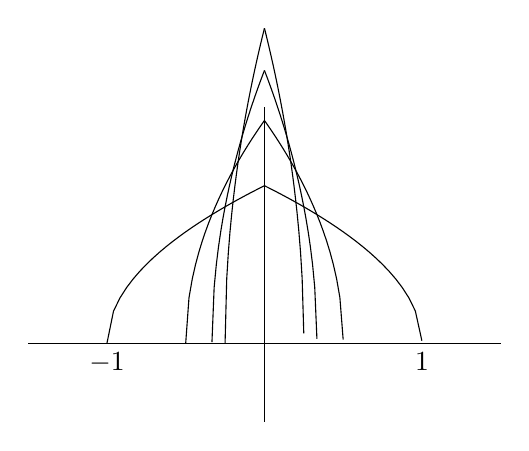
\begin{tikzpicture}[scale=2]
        \draw (-1.5,0) -- (1.5,0);
        \draw (0,-0.5) -- (0,1.5);
        \node [below] at (-1,0) {$-1$};
        \node [below] at (1,0) {$1$};
        \draw [domain=-1:0] plot ({\x},{sqrt(1+\x)});
        \draw [domain=-1/2:0] plot ({\x},{sqrt(2+4*\x)});
        \draw [domain=-1/3:0] plot ({\x},{sqrt(3+9*\x)});
        \draw [domain=-1/4:0] plot ({\x},{sqrt(4+16*\x)});
        \draw [domain=0:1] plot ({\x},{sqrt(1-\x)});
        \draw [domain=0:1/2] plot ({\x},{sqrt(2-4*\x)});
        \draw [domain=0:1/3] plot ({\x},{sqrt(3-9*\x)});
        \draw [domain=0:1/4] plot ({\x},{sqrt(4-16*\x)});
      \end{tikzpicture}
    \end{minipage}

    \begin{minipage}{4in}
      Let $\abs{f_n(t)}^2=\begin{cases}
      0, & -1\le t\le-\frac{1}{n} \\
      n+n^2t, & -\frac{1}{n}\le t\le0 \\
      n-n^2t, & 0\le t\le\frac{1}{n} \\
      0, & \frac{1}{n}\le t\le-1
      \end{cases}$
    \end{minipage}
    \begin{minipage}{3in}
      \begin{tikzpicture}[scale=2]
        \draw (-1.5,0) -- (1.5,0);
        \draw (0,-0.5) -- (0,4.5);
        \node [below] at (-1,0) {$-1$};
        \node [below] at (1,0) {$1$};
        \draw [domain=-1:0] plot ({\x},{1+\x});
        \draw [domain=-1/2:0] plot ({\x},{2+4*\x});
        \draw [domain=-1/3:0] plot ({\x},{3+9*\x});
        \draw [domain=-1/4:0] plot ({\x},{4+16*\x});
        \draw [domain=0:1] plot ({\x},{1-\x});
        \draw [domain=0:1/2] plot ({\x},{2-4*\x});
        \draw [domain=0:1/3] plot ({\x},{3-9*\x});
        \draw [domain=0:1/4] plot ({\x},{4-16*\x});
      \end{tikzpicture}
    \end{minipage}

    $\norm{f_n}=1$
    But $f_n\to\delta_0\notin\mc[-1,1]$ (Dirac-Delta)
  \end{enumerate}
\end{examples}

\end{document}
